% !TEX TS-program = pdflatex
% !TEX encoding = UTF-8 Unicode

% This file is a template using the "beamer" package to create slides for a talk or presentation
% - Talk at a conference/colloquium.
% - Talk length is about 20min.
% - Style is ornate.

% MODIFIED by Jonathan Kew, 2008-07-06
% The header comments and encoding in this file were modified for inclusion with TeXworks.
% The content is otherwise unchanged from the original distributed with the beamer package.

\documentclass{beamer}


% Copyright 2004 by Till Tantau <tantau@users.sourceforge.net>.
%
% In principle, this file can be redistributed and/or modified under
% the terms of the GNU Public License, version 2.
%
% However, this file is supposed to be a template to be modified
% for your own needs. For this reason, if you use this file as a
% template and not specifically distribute it as part of a another
% package/program, I grant the extra permission to freely copy and
% modify this file as you see fit and even to delete this copyright
% notice. 


\mode<presentation>
{
  \usetheme{Warsaw}
  % or ...

  \setbeamercovered{transparent}
  % or whatever (possibly just delete it)
}


\usepackage[english]{babel}
% or whatever

\usepackage[utf8]{inputenc}
% or whatever

\usepackage{times}
\usepackage[T1]{fontenc}
% Or whatever. Note that the encoding and the font should match. If T1
% does not look nice, try deleting the line with the fontenc.
 \newcommand{\abs}[1]{\left|{#1}\right|}
 \newcommand{\av}[1]{\left\langle #1 \right\rangle}
 
  \newcommand{\br}[1]{\langle #1|}
  \newcommand{\ke}[1]{|#1\rangle}
  \newcommand{\bk}[2]{\langle #1|#2\rangle}
  \newcommand{\kb}[2]{\ke{#1}\br{#2}}
  \newcommand{\var}[2]{\langle #1|#2\rangle} 
  \newcommand{\ov}[2]{\abs{\var{#1}{#2}}^2}
\newcommand{\td}[1]{\widetilde{#1}}

%\title[Short Paper Title] % (optional, use only with long paper titles)
%{Second Examination}

\title
{Optimal Measurements Tasks and Their Physical Realizations}

\author[Vadim Yerokhin] % (optional, use only with lots of authors)
{Vadim Yerokhin }
% - Give the names in the same order as the appear in the paper.
% - Use the \inst{?} command only if the authors have different
%   affiliation.

% - Use the \inst command only if there are several affiliations.
% - Keep it simple, no one is interested in your street address.

\date[CFP 2003] % (optional, should be abbreviation of conference name)
{Hunter College, August 17th 2015 }
% - Either use conference name or its abbreviation.
% - Not really informative to the audience, more for people (including
%   yourself) who are reading the slides online


% If you have a file called "university-logo-filename.xxx", where xxx
% is a graphic format that can be processed by latex or pdflatex,
% resp., then you can add a logo as follows:

% \pgfdeclareimage[height=0.5cm]{university-logo}{university-logo-filename}
% \logo{\pgfuseimage{university-logo}}



% Delete this, if you do not want the table of contents to pop up at
% the beginning of each subsection:
\AtBeginSubsection[]
{
  \begin{frame}<beamer>{Outline}
    \tableofcontents[currentsection,currentsubsection]
  \end{frame}
}


% If you wish to uncover everything in a step-wise fashion, uncomment
% the following command: 

%\beamerdefaultoverlayspecification{<+->}


\begin{document}

\begin{frame}
  \titlepage
\end{frame}

\begin{frame}{Outline}
  \tableofcontents[pausesections]
  % You might wish to add the option [pausesections]
\end{frame}


% Structuring a talk is a difficult task and the following structure
% may not be suitable. Here are some rules that apply for this
% solution: 

% - Exactly two or three sections (other than the summary).
% - At *most* three subsections per section.
% - Talk about 30s to 2min per frame. So there should be between about
%   15 and 30 frames, all told.

% - A conference audience is likely to know very little of what you
%   are going to talk about. So *simplify*!
% - In a 20min talk, getting the main ideas across is hard
%   enough. Leave out details, even if it means being less precise than
%   you think necessary.
% - If you omit details that are vital to the proof/implementation,
%   just say so once. Everybody will be happy with that.

%%%%%%%%%%%%%%%%%%%%%%%%%%%%%%%%%%%%%%%%%%%%%%%%
%%%%%%%%%%%%%%%%%%%%%%%%%%%%%%%%%%%%%%%%%%%%%%%%
\section{Introduction}
\subsection{Information Theory}
\begin{frame}{Motivation}
\begin{itemize}
\item
Classical bits versus quantum bits: instead of just a 0 or 1, quantum bits can maintain a superposition state of both
\pause
\item
Quantum computing-Shor's algoritm allows cracking of modern communications security based on prime decomposition
\pause
\item
Quantum communication- B92 protocol allows for completely secure communication
\end{itemize}
\end{frame}
%%%%%%%%%%%%%%%%%%%%%%%%%%%%%%%%%%%%%%%%%%%%%%%%
%%%%%%%%%%%%%%%%%%%%%%%%%%%%%%%%%%%%%%%%%%%%%%%%
\begin{frame}{Our Games}
\begin{itemize}
\item
Someone prepares one of two different pure states $\ke {\psi_i} = \alpha_i \ke 0 +  \beta_i \ke 1$
or one of two ensembles $\rho_i = \sum_i c_i \kb{\psi_i}{\psi_i}$, for $i = 1,2$.
\pause
\item
Each outcome has a different likelihood $\eta_i$ that sum to 1.
\pause
\item
One particle (state) is sent at a time.  Our job is to:
\begin{itemize}
\item
 Guess as best we can what state was sent (discrimination)
\item Make the state more orthogonal to its complement (separation)
\item
Make copies of the input state (cloning)

\end{itemize}

\end{itemize}

\end{frame}

%%%%%%%%%%%%%%%%%%%%%%%%%%%%%%%%%%%%%%%%%%%%%%%%
%%%%%%%%%%%%%%%%%%%%%%%%%%%%%%%%%%%%%%%%%%%%%%%%
\begin{frame}{Unitary Time Evolution}
The Schrodinger equation for ensembles is
\[i \hbar \frac{\partial\rho}{\partial t} =  [H,\rho].\]
Solving this for evolution of initial state $\rho(t=0)$ we get
\[\rho(t) = U(t) \rho(0) U(t)^\dagger\]
 where the unitary matrix U obeys $UU^\dagger = I$.
There are several ways to view this formula.
\end{frame}
%%%%%%%%%%%%%%%%%%%%%%%%%%%%%%%%%%%%%%%%%%%%%%%%
%%%%%%%%%%%%%%%%%%%%%%%%%%%%%%%%%%%%%%%%%%%%%%%%
\begin{frame}{Neumark's theorem}
\begin{itemize}
\item
The first is as the time evolution of a pure system evolving with pure ancilla
\[U(\ke {\psi_A} \otimes \ke {\phi_B}) = \sum_i A_i \ke {\psi_A} \otimes \ke {i_B}.\]
using the  Kraus operators $A_i$ such that $\sum A_i A_i^\dagger = \sum \Pi_i = I$,
the $\Pi_i$'s representing different measurement outcomes.

\item
The other is simply as a unitary acting on a pure state $\psi$ to make state $\phi$, as in $U\ke \psi = \ke \phi$.
\end{itemize}
\end{frame}
%%%%%%%%%%%%%%%%%%%%%%%%%%%%%%%%%%%%%%%%%%%%%%%%
%%%%%%%%%%%%%%%%%%%%%%%%%%%%%%%%%%%%%%%%%%%%%%%%
\subsection{Pure State Discrimination Strategies}

\begin{frame}{No-go}
If perfect discrimination were possible we could write it as
\[\Pi_1 \ke {\psi_2} = 0,\]
\[\Pi_2 \ke {\psi_1} = 0,\]
then using $\Pi_1 + \Pi_2 = I$ and the inner product of these equations, we get the same result:
\[0= \br{\psi_2} \Pi_1 + \Pi_2 \ke {\psi_1} = \bk{\psi_1}{\psi_2} \]
 Since the two constraints of measurement,
orthogonality of the measurement vectors and their spanning the space, proved contradictory, we must give up one of these two
functions in order to perform a physical measurement.
\end{frame}
%%%%%%%%%%%%%%%%%%%%%%%%%%%%%%%%%%%%%%%%%%%%%%%%
%%%%%%%%%%%%%%%%%%%%%%%%%%%%%%%%%%%%%%%%%%%%%%%%
\begin{frame}{Minimum Error Discrimination (ME)}
\begin{itemize}
\item
	Two orthogonal projectors, each clicks for a state.
\pause
\item
	There is a success rate and an error rate if the states are not orthogonal.
\[ P_s =\eta_1 Tr(\rho_1 \Pi_1) + \eta_2Tr(\rho_2 \Pi_2)\]
\[ P_e = \eta_2 Tr(\rho_2 \Pi_1) +\eta_1 Tr(\rho_1 \Pi_2)\]
\pause
\item
	The minimum error rate for pure states is achieved by the Helstrom bound.
\[P_E = \frac{1}{2}(1- \sqrt{1-4 \eta_1 \eta_2 \ov{\psi_1}{\psi_2}})\]
\end{itemize}
\end{frame}
%%%%%%%%%%%%%%%%%%%%%%%%%%%%%%%%%%%%%%%%%%%%%%%%
%%%%%%%%%%%%%%%%%%%%%%%%%%%%%%%%%%%%%%%%%%%%%%%%
\begin{frame}{Minimum Error Graph}
\begin{figure}[th]
\centering
$%
\begin{array}{c}
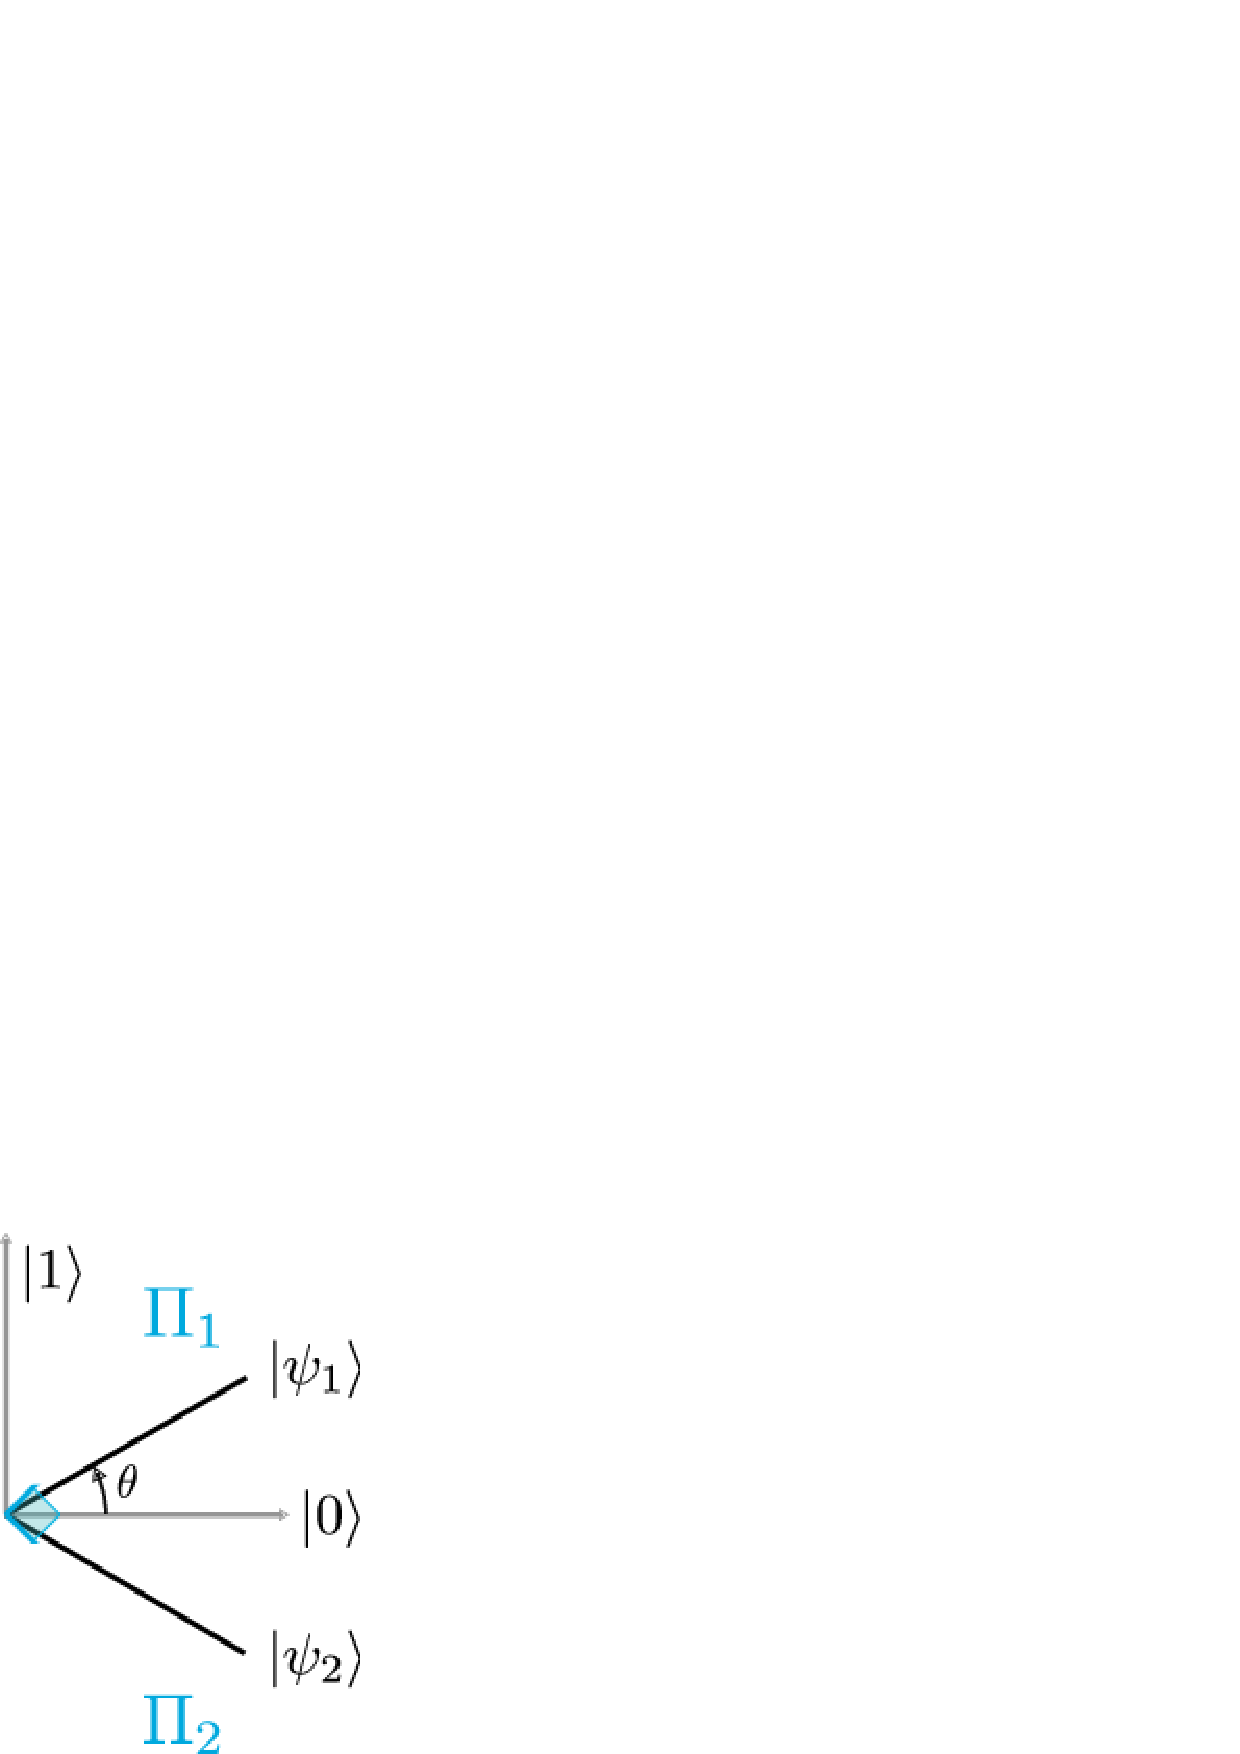
\includegraphics[height=6 cm]{ME.png} \\

\end{array}%
$%

\label{fig:Graphs}
\end{figure}
\end{frame}
%%%%%%%%%%%%%%%%%%%%%%%%%%%%%%%%%%%%%%%%%%%%%%%%
%%%%%%%%%%%%%%%%%%%%%%%%%%%%%%%%%%%%%%%%%%%%%%%%
\begin{frame}{Unambigious State Discrimination (UD)}



\begin{itemize}
\pause
\item
	Make the measurement operators orthogonal to the state that we don't want to measure.
\pause
\item
	Since they are no longer orthogonal they don't sum to the identity. A third, inconclusive outcome is necessary.
\item
	The detector corresponding to the inconclusive outcome we call $\Pi_0$.
\pause

\item
	The failure probability we call Q:

\[Q =  \eta_1 Tr(\rho_1 \Pi_0) +\eta_2  Tr(\rho_2 \Pi_0) = Tr(\rho \Pi_0).\]
\pause
\item
$ Q_0 = 2 \sqrt{\eta_1\eta_2} cos \theta$  is the failure rate that corresponds to the best measurement.
\end{itemize}

\end{frame}
%%%%%%%%%%%%%%%%%%%%%%%%%%%%%%%%%%%%%%%%%%%%%%%%
%%%%%%%%%%%%%%%%%%%%%%%%%%%%%%%%%%%%%%%%%%%%%%%%
\begin{frame}{Unambiguous State Discrimination Graph}
\begin{figure}[th]
\centering
$%
\begin{array}{c}
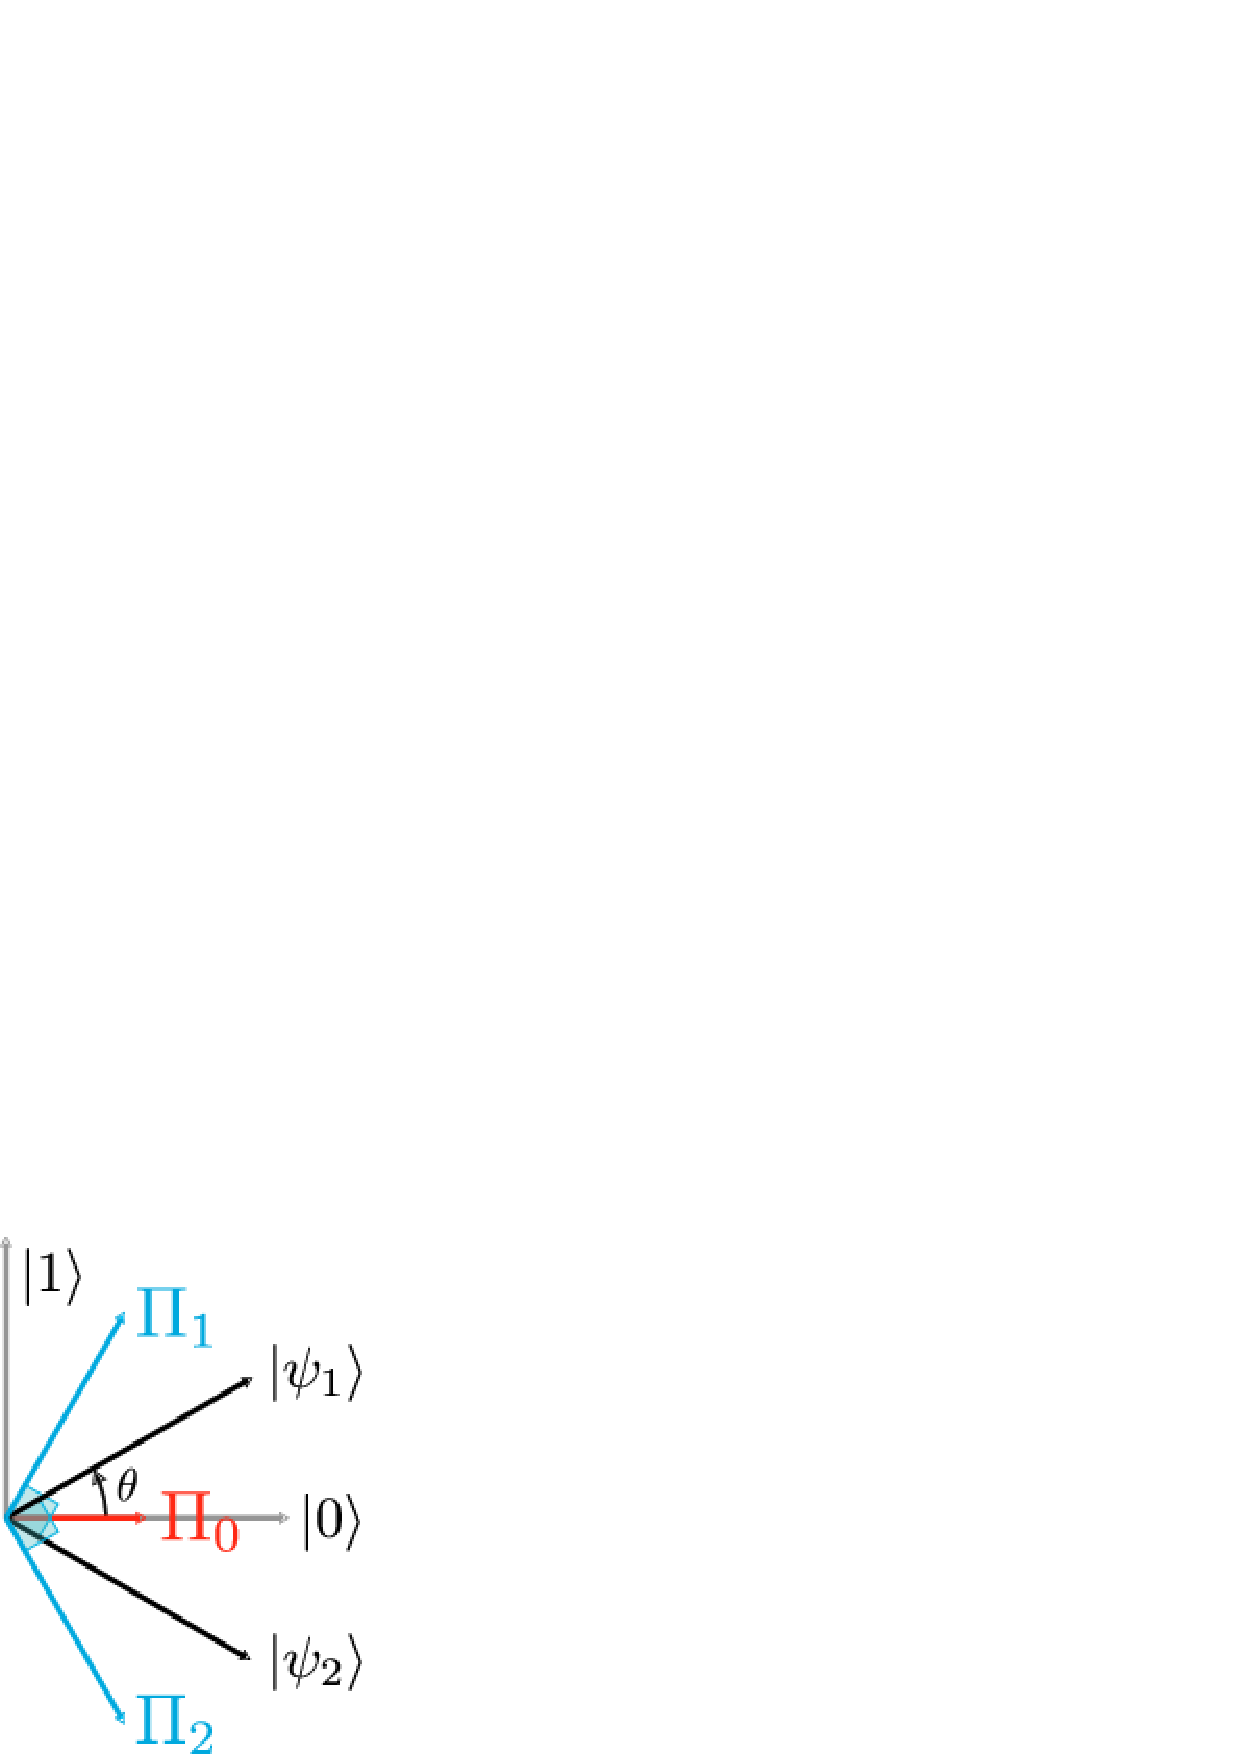
\includegraphics[height=6 cm]{UD.png} \\

\end{array}%
$%

\label{fig:Graphs}
\end{figure}
\end{frame}
%%%%%%%%%%%%%%%%%%%%%%%%%%%%%%%%%%%%%%%%%%%%%%%%
%%%%%%%%%%%%%%%%%%%%%%%%%%%%%%%%%%%%%%%%%%%%%%%%

\begin{frame}{Intermediate Discrimination (IM)}
\begin{figure}[th]
\centering
$%
\begin{array}{c}
\includegraphics[height=6 cm]{IM.png} \\

\end{array}%
$%

\label{fig:Graphs}
\end{figure}

\end{frame}
%%%%%%%%%%%%%%%%%%%%%%%%%%%%%%%%%%%%%%%%%%%%%%%%
%%%%%%%%%%%%%%%%%%%%%%%%%%%%%%%%%%%%%%%%%%%%%%%%
\begin{frame}{Lagrange Multipliers method}
We can cast the problem via Neumark's theorem as
\begin{eqnarray*}
U \ke {\psi_1}= \sqrt{p_1} \ke 1 + \sqrt{r_1} \ke 2 + \sqrt{q_1} \ke 0, \\
U |\psi_2 \rangle = \sqrt{r_2} \ke 1 + \sqrt{p_2} \ke 2 + \sqrt{q_2} \ke 0.
\end{eqnarray*}

The inner product of these two equations is useful. We call it the unitarity constraint:
\[s = \langle\psi_1|\psi_2\rangle\ = \sqrt{p_1 r_2} + \sqrt{p_2 r_1} + \sqrt{q_1 q_2}.\]
\end{frame}
%%%%%%%%%%%%%%%%%%%%%%%%%%%%%%%%%%%%%%%%%%%%%%%%
%%%%%%%%%%%%%%%%%%%%%%%%%%%%%%%%%%%%%%%%%%%%%%%%
\begin{frame}
We now use the Lagrange multiplier method to minimize $P_e$ subject to the inner-product constraint and fixed failure rate Q.
\[F_e = \eta_1 r_1 + \eta_2 r_2 + \lambda (s - \rm Unitarity\hspace{.1 cm}Constraint ).\]
A lot of algebra gives us the optimal individual error rates as:

\[r_1=\frac{1}{2}[\alpha_1-\frac{[2\eta_2\omega-\alpha_1(1-Q)]}{\sqrt{(1-Q)^2-4\omega\eta_1\eta_2}}]\]
and
\[r_2=\frac{1}{2}[\alpha_2-\frac{[2\eta_1\omega-\alpha_2(1-Q)]}{\sqrt{(1-Q)^2-4\omega\eta_1\eta_2}}]\]
where $\alpha_i \equiv 1-q_i $ and  $\omega\equiv(s -\sqrt{q_1 q_2})^2$ and finally
\[ P_e = \frac{1}{2} (1 - Q -\sqrt{(1-Q)^2 - (Q-Q_0)^2}),\]
\end{frame}

%%%%%%%%%%%%%%%%%%%%%%%%%%%%%%%%%%%%%%%%%%%%%%%%
%%%%%%%%%%%%%%%%%%%%%%%%%%%%%%%%%%%%%%%%%%%%%%%%
\begin{frame}
We've solved some state discrimination problems involving mixed states but we've presented the results before so we move on to other,
more interesting topics!
\end{frame}

\begin{frame}
We can consider an operation such as UD or IM as a two-step measurement.  
\begin{itemize}
\item
In the first step we probabilistically separate the states.  
\item
In the second step, if the first was successful, orthogonal detection operators (ME) discriminate the states.
\end{itemize}
\[\]
What if we only wanted to perform the first step?
\end{frame}

%%%%%%%%%%%%%%%%%%%%%%%%%%%%%%%5
%%%%%%%%%%%%%%%%%%%%%%%%%%%%%%%%%%
%%%%%%%%%%%%%%%%%%%%%%%%%%%%%%%5
%%%%%%%%%%%%%%%%%%%%%%%%%%%%%%%%%%
%%%%%%%%%%%%%%%%%%%%%%%%%%%%%%%5
%%%%%%%%%%%%%%%%%%%%%%%%%%%%%%%%%%
\section{State Separation}
\begin{frame}
We want to make the pure states $\psi_i$ probabilistically more distinguishable, via
equations
\begin{eqnarray*}
U|\psi_{1}\rangle|0\rangle & = & \sqrt{p_{1}}|\phi_{1}\rangle|1\rangle+\sqrt{q_{1}}\ke 0,\nonumber \\
U|\psi_{2}\rangle|0\rangle & = & \sqrt{p_{2}}|\phi_{2}\rangle|1\rangle+\sqrt{q_{2}}\ke 0.
\end{eqnarray*}
Here the inner product equation is $s = \sqrt{p_1 p_2} s' + \sqrt{q_1 q_2}$ where $s' = \bk{\phi_1}{\phi_2}$.

\end{frame}
%%%%%%%%%%%%%%%%%%%%%%%%%%%%%%%5
%%%%%%%%%%%%%%%%%%%%%%%%%%%%%%%%%%
\begin{frame}
A particularly attractive geometric formulation of this constraint comes from
choosing the change of variables 
$u\equiv\sqrt{q_{1}q_{2}},\hspace{0.3cm}v\equiv\frac{1}{2}\left(q_{1}+q_{2}\right)$.
\begin{itemize}
\item
The unitarity constraint becomes parabola $v={1+u^2\over2}-{(u-s)^2\over2s'^2}$.
\item
The failure rate curve beomces parametrized ellipse

\begin{eqnarray}
u&=&{Q\over\sqrt{1-\Delta^2}}\cos\theta,\nonumber\\
v&=&{Q\over1-\Delta^2}+{Q\Delta\over1-\Delta^2}\sin\theta,
\end{eqnarray}
\end{itemize}
where $\Delta = \eta_2 - \eta_1$.
Then both the failure rate and unitarity constraint become conic sections (an ellipse and parabola).  The optimality
condition is their tangency, and we are able to derive all bounds parametrically.
\end{frame}
%%%%%%%%%%%%%%%%%%%%%%%%%%%%%%%5
%%%%%%%%%%%%%%%%%%%%%%%%%%%%%%%%%%
\begin{frame}
\begin{figure}[th]
\centering
$%
\begin{array}{c}
\includegraphics[height=7 cm]{Figures_SEPvedit.pdf} \\

\end{array}%
$%

\label{fig:Graphs}
\end{figure}


\end{frame}


%%%%%%%%%%%%%%%%%%%%%%%%%%%%%%%5
%%%%%%%%%%%%%%%%%%%%%%%%%%%%%%%%%%
%%%%%%%%%%%%%%%%%%%%%%%%%%%%%%%5
%%%%%%%%%%%%%%%%%%%%%%%%%%%%%%%%%%
%%%%%%%%%%%%%%%%%%%%%%%%%%%%%%%5
%%%%%%%%%%%%%%%%%%%%%%%%%%%%%%%%%%
\section{Cloning Pure States}

\begin{frame}{No-go}
Suppose we wrote the equations describing the unitary that cloned one of two input pure states $\psi_i$ with
a-priori probabilities $\eta_i$ for $i = 1,2$.  If we could perform this measurement perfectly we would write
\begin{eqnarray}
U\ke{\psi_1}\ke 0 = \ke{\psi_1}\ke{\psi_1},\\
U\ke{\psi_2}\ke 0 = \ke{\psi_2}\ke{\psi_2}.
\end{eqnarray}
However, taking the inner product of the two equations we find $\bk{\psi_1}{\psi_2} = \bk{\psi_1}{\psi_2}^2$,
restricting the functionality of this unitary to the trivial case when the two states are orthogonal and $\bk{\psi_1}{\psi_2}=0$.
Therefore there does not exist in general a unitary to perform this ideal cloning task.  As with state discrimination, 
we must choose a figure of merit to maximize.
\end{frame}
%%%%%%%%%%%%%%%%%%%%%%%%%%%%%%%5
%%%%%%%%%%%%%%%%%%%%%%%%%%%%%%%%%%%%%%%%%%%%%%%%%%%%%%%%%%%%%%%%%5
%%%%%%%%%%%%%%%%%%%%%%%%%%%%%%%%%%
\subsection{Deterministic Approximate Cloning}
\begin{frame}
The 'minimum error' cloning method was devised by Chefles and Barnett to make two imperfect copies of one of two input states.
The unitary representation of this transformation is
\begin{eqnarray*}
U \ke{\psi_1}\ke 0  = \ke {\phi_1}\ke{\phi_1}\\
U \ke{\psi_2}\ke 0  = \ke {\phi_2}\ke{\phi_2}
\end{eqnarray*}
Where we want to maximize is the average fidelity
\[F = \eta_1 \bk{\psi_1}{\phi_1}^2 +\eta_2 \bk{\psi_2}{\phi_2}^2\]
The optimal fidelity is
\[F = \frac{1}{2}( 1 + \sqrt{1-  4 \eta_1 \eta_2 \sin^2 2\alpha}).\]
where $\alpha = \theta -\frac{\phi_1 - \phi_2}{2}$.
\end{frame}
%%%%%%%%%%%%%%%%%%%%%%%%%%%%%%%5
%%%%%%%%%%%%%%%%%%%%%%%%%%%%%%%%%%%%%%%%%%%%%%%%%%%%%%%%%%%%%%%%%5
%%%%%%%%%%%%%%%%%%%%%%%%%%%%%%%%%%
\subsection{Probabilistic Exact Cloning}
\begin{frame}
Here we take 'unambiguous' method to solving the problem and sometimes make perfect clones.  We consider $m$ input states turned into $n$ output states.
\begin{equation*}
U|\psi^m_i\rangle|0\rangle= \sqrt{p_i}|\psi^n_i\rangle|1\rangle +\sqrt q_i |\Phi\rangle |0\rangle,\quad i=1,2. \label{Ui}
\end{equation*}

The overlap equation now reads 
\[s^m = \bk {\psi_1^m}{\psi_2^m} = \sqrt{p_1 p_2} \bk {\psi_1^n}{\psi_2^n}  + \sqrt{q_1 q_2} =\sqrt{p_1 p_2} s^n+ \sqrt{q_1 q_2}.\]

If at this point you think this equation looks remarkably similar to everything else, you'd be right. But particularly to the separation
 unitarity condition with $s \rightarrow s^M$,$s' \rightarrow s^N$.
\href{file:///C:/Users/Vadim/Documents/work/Final exam/manipulateUnitaryCondition.swf}{Load Clip}
\end{frame}


%%%%%%%%%%%%%%%%%%%%%%%%%%%%%%%5
%%%%%%%%%%%%%%%%%%%%%%%%%%%%%%%%%%%%%%%%%%%%%%%%%%%%%%%%%%%%%%%%%5
\begin{frame}{Geometric Picture}


We want optimize the success rate given the unitary curve
\[s^m=\sqrt{p_1 p_2} s^n+ \sqrt{q_1 q_2}\]
 and subject to a fixed failure rate 
\[Q = \eta_1 q_1 + \eta_2 q_2.\] 
In the $q_1$ vs $q_2$ coordinate system, these two equations appear as a complex curve and a straight line.  To satisfy both conditions means the curves must intersect.
It can be proven that tangency is the requirement. 
\end{frame}

%%%%%%%%%%%%%%%%%%%%%%%%%%%%%%%5
%%%%%%%%%%%%%%%%%%%%%%%%%%%%%%%%%%%%%%%%%%%%%%%%%%%%%%%%%%%%%%%%%5
\begin{frame}
\begin{figure}[t]
\centering
\includegraphics[width=14em]{Figures_CLONEvedit.pdf}
%
\caption{ The figure shows the overlap constraint and the optimal straight segment \mbox{$Q=\eta_1 q_1+\eta_2 q_2$} and its normal vector~$(\eta_1,\eta_2)$. Plotted for  $s = 0.6$, $\eta_1=0.17$, $\eta_2=0.83$ and~$Q=0.24$.}
\label{fig:1}
\end{figure}
\end{frame}
%%%%%%%%%%%%%%%%%%%%%%%%%%%%%%%5
%%%%%%%%%%%%%%%%%%%%%%%%%%%%%%%%%%%%%%%%%%%%%%%%%%%%%%%%%%%%%%%%%5
\begin{frame}{Parametrization}
We use the change of variables $\sqrt{q_i} = \sin \theta_i$ then $x = cos(\theta_1 + \theta_2)$, $y = (cos\theta_1 -\theta_2)$ to write the unitary constraint as
\[x=\frac{1-(1+s^n)t}{s^{n-m}},\qquad y=\frac{1-(1-s^n)t}{s^{n-m}}.\]
In this form we can write the failure rates as
\begin{equation}
q_i=\frac{1-xy-(-1)^i\sqrt{1-x^2}\sqrt{1-y^2}}{2}.
\end{equation}
\end{frame}
%%%%%%%%%%%%%%%%%%%%%%%%%%%%%%%5
%%%%%%%%%%%%%%%%%%%%%%%%%%%%%%%%%%%%%%%%%%%%%%%%%%%%%%%%%%%%%%%%%5
\begin{frame}{Optimization}
We can characterize our result by expressing the necessery a-priori $\eta_i$ for any point on the unitary curve.  These take the form
\begin{equation*}
\eta_1=\frac{q'_2}{q'_2-q'_1},\;\; Q_{\rm min}=\frac{q'_2 q_1-q'_1 q_2}{q'_2-q'_1},\;\; t_{-1}\le t\le t_0,
\label{main}
\end{equation*}
where the derivative of $q$ is
\begin{equation}
q'_i=\frac{\sqrt{q_i(1-q_i)}}{s^{n-m}}\left\{\frac{1+s^n}{\sqrt{1-x^2}}-(-1)^i\frac{1-s^n}{\sqrt{1-y^2}}\right\}.
\end{equation}
\end{frame}
%%%%%%%%%%%%%%%%%%%%%%%%%%%%%%%5
%%%%%%%%%%%%%%%%%%%%%%%%%%%%%%%%%%%%%%%%%%%%%%%%%%%%%%%%%%%%%%%%%5
\begin{frame}{Relation to State Discrimination}
\begin{figure}[ht]
$%
\begin{array}{c}
\includegraphics[width=26.7em]{Fig_3NC.pdf}\\
\end{array}%
$%

\end{figure}
\end{frame}
%%%%%%%%%%%%%%%%%%%%%%%%%%%%%%%5
%%%%%%%%%%%%%%%%%%%%%%%%%%%%%%%%%%%%%%%%%%%%%%%%%%%%%%%%%%%%%%%%%5
\begin{frame}
Optimal cloning is always better than discrimination, though this difference decreases with more clones.  In the limit $n \rightarrow \infty$ there is perfect agreement.
In geometric terms, the unitary curve $s^m=\sqrt{p_1 p_2} s^n+ \sqrt{q_1 q_2}$ collapses onto the hyperbola $s^m =  \sqrt{q_1 q_2}$, which is the constraint for 
UD state discrimination.  Therefore the limiting solution to our cloning procedure is unambiguous discrimination.
\end{frame}
%%%%%%%%%%%%%%%%%%%%%%%%%%%%%%%5
%%%%%%%%%%%%%%%%%%%%%%%%%%%%%%%%%%%%%%%%%%%%%%%%%%%%%%%%%%%%%%%%%5
\subsection{Intermediate Cloning}
\begin{frame}
Chefles and Barnett solved the equal priors case in 1998, giving us the optimal global fidelity as 
\[F_{MN} = \frac{1}{2}\left[1+|\langle\psi_{1}^{N}|\psi_{2}^{N}\rangle|\left(1-\frac{P_{IDP}}{P_{S}}\right)\right]+\]
\[\frac{1}{2 P_{S}}(\left(1-|\langle\psi_{1}^{N}|\psi_{2}^{N}\rangle|^{2}\right)\left(P_{S}^{2}-\left(P_{S}-P_{IDP}\right)^{2}\right)^{1/2}\]
As you may imagine the unequal priors case cannot be solved in the same manner.  This formula reduces to intermediate discrimination in the $n \rightarrow \infty$ limit.

\end{frame}

%%%%%%%%%%%%%%%%%%%%%%%%%%%%%%%5
%%%%%%%%%%%%%%%%%%%%%%%%%%%%%%%%%%%%%%%%%%%%%%%%%%%%%%%%%%%%%%%%%5
\begin{frame}{Arbitrary Priors}
This takes two steps: first maximally separate the incoming states for a fixed rate of inconclusive result, 
\begin{itemize}
\item Step 1: State Separation
\end{itemize}
Optimally separate the incoming states $\left\{ \ke{\psi_{1}^{M}},\ke{\psi_{2}^{M}}\right\} $
with a fixed rate of inconclusive results $q_{i}$, then prepare states
$\left\{ \ke{\Psi_{1}},\ke{\Psi_{2}}\right\} $ with the
corresponding success probabilities. 

The incoming states are separated with a success probability $p_{i}$
and failed to separate the states with a failure probability $q_{i}$.
\end{frame}
%%%%%%%%%%%%%%%%%%%%%%%%%%%%%%%5
%%%%%%%%%%%%%%%%%%%%%%%%%%%%%%%%%%%%%%%%%%%%%%%%%%%%%%%%%%%%%%%%%5
\begin{frame}
\begin{itemize}
\item Step 2: Optimize Deterministic Fidelity
\end{itemize}
The resulting states are rotated in such a way that their average overlap with n copies of the original state is mazimized. 
More precisely, for individual fidelities $F_i = |\bk{\psi_i^N}{\phi_i}|^2$ we want to maximize the global conditional fidelilty 
\[F = \frac{\eta_1 p_1 F_1 + \eta_2 p_2 F_2}{1-Q} = \tilde{\eta_1} F_1 + \tilde{\eta_2} F_2\]
Where we've also shown the resulting normalization.  This normalization means we can apply the deterministic fidelity result to this problem.
\end{frame}
%%%%%%%%%%%%%%%%%%%%%%%%%%%%%%%5
%%%%%%%%%%%%%%%%%%%%%%%%%%%%%%%%%%%%%%%%%%%%%%%%%%%%%%%%%%%%%%%%%5
\begin{frame}
The resulting fidelity expression,
\[F_{MN}  = \frac{1}{2}\left[1+\sqrt{1-4\tilde{\eta}_{1}\tilde{\eta}_{2}\sin^{2}\left(2\theta-\left(\phi_{1}+\phi_{2}\right)\right)}\right],\]
  has a remaining optimization under the square root, namely the term
\begin{equation*}
\Lambda =  \sqrt{p_{1}p_{2}}\sin\left(2\theta-\left(\phi_{1}+\phi_{2}\right)\right).
\end{equation*}
can be written with optimal separation as
\begin{equation*}
\Lambda = \sqrt{1-s^{2n}}\left(s-u\right)-s^{n}\sqrt{1-s^{2}-2v+2sv}
\end{equation*}
where $u\equiv\sqrt{q_{1}q_{2}},\hspace{0.3cm}v\equiv\frac{1}{2}\left(q_{1}+q_{2}\right)$, 
are variables we will introduce in the next section on state separation.
\end{frame}
%%%%%%%%%%%%%%%%%%%%%%%%%%%%%%%5
%%%%%%%%%%%%%%%%%%%%%%%%%%%%%%%%%%
%%%%%%%%%%%%%%%%%%%%%%%%%%%%%%%5
%%%%%%%%%%%%%%%%%%%%%%%%%%%%%%%%%%
%%%%%%%%%%%%%%%%%%%%%%%%%%%%%%%5
%%%%%%%%%%%%%%%%%%%%%%%%%%%%%%%%%%
\section{Linear Optical Implementations}
\begin{frame}
Every unitary can be reduced into beam splitters and phase-shifters via the
Reck-Zeilinger algorithm.  This has been experimentally implemented for various protocols.

\begin{figure}[th]
\centering
$%
\begin{array}{c}
\includegraphics[height=5.5 cm]{Separation_F5.pdf} \\

\end{array}%
$%

\label{fig:Graphs}
\end{figure}

\end{frame}
%%%%%%%%%%%%%%%%%%%%%%%%%%%%%%%5
%%%%%%%%%%%%%%%%%%%%%%%%%%%%%%%%%%%%%%%%%%%%%%%%%%%%%%%%%%%%%%%%%5
\begin{frame}{Approximate Probabilistic Cloning}
We can decompose the action of a probabilistic cloner into two steps,
first separate the states and then clone them to the desired copies.  We will show
this setup for equal prior probabilities.
\end{frame}
%%%%%%%%%%%%%%%%%%%%%%%%%%%%%%%5
%%%%%%%%%%%%%%%%%%%%%%%%%%%%%%%%%%%%%%%%%%%%%%%%%%%%%%%%%%%%%%%%%5
\begin{frame}{Separation}
\begin{eqnarray}
U\ke {\psi_1} = \sqrt{p_1}\ke{\phi_1}+ \sqrt{q_1}\ke{0}\\
U\ke {\psi_2} = \sqrt{p_2}\ke{\phi_2}+ \sqrt{q_2}\ke{0}
\end{eqnarray}
where $\ke {\psi_1} = c_1 \ke{1} + s_1 \ke{2}$,
$\ke {\psi_2} = c_1 \ke{1} - s_1 \ke{2}$,
$\ke {\phi_1} = c_2 \ke{1} + s_2 \ke{2}$,
$\ke {\phi_2} = c_2 \ke{1} - s_2 \ke{2}$.
then we get the equations
\begin{eqnarray}
\br 0 U \ke {\psi_1} &=&c_1 U_{01} + s_1 U_{02} = \sqrt{q_1}\\
\br 1 U \ke {\psi_1} &=&c_1 U_{11} + s_1 U_{12} = c_2 \sqrt{p_1}\\
\br 2 U \ke {\psi_1} &=&c_1 U_{21} + s_1 U_{22} = s_2\sqrt{p_1}
\end{eqnarray}
\end{frame}
%%%%%%%%%%%%%%%%%%%%%%%%%%%%%%%5
%%%%%%%%%%%%%%%%%%%%%%%%%%%%%%%%%%%%%%%%%%%%%%%%%%%%%%%%%%%%%%%%%5
\begin{frame}
Using the optimal sucess rate 
\begin{equation}
p = \frac{\bk{\psi_1}{\psi_2}-1}{\bk{\phi_1}{\phi_2}-1},
\end{equation}
 we can choose the remaining elements to be
\begin{equation}
{}[U]=
\begin{pmatrix}\frac{c_2s_1}{c_1s_2}& \frac{\sqrt{s_2^2-s_1^2}}{c_1s_2} & 0\\
-\frac{\sqrt{s_2^2-s_1^2}}{c_1s_2} &\frac{c_2s_1}{c_1s_2} & 0 \\
0 & 0 & 1
\end{pmatrix}
\end{equation}
and only one beam splitter is needed to perform this operation.
\end{frame}
%%%%%%%%%%%%%%%%%%%%%%%%%%%%%%%5
%%%%%%%%%%%%%%%%%%%%%%%%%%%%%%%%%%%%%%%%%%%%%%%%%%%%%%%%%%%%%%%%%5
\begin{frame}{Deterministic Cloning}
The unitary transformation
for the second step is
\begin{eqnarray}
U\ke {\phi_1} \ke 0 = \ke{\xi_1}\ke{\xi_1}\\
U\ke {\phi_2} \ke 0 = \ke{\xi_2}\ke{\xi_2}
\end{eqnarray}
where 
$\ke {\xi_1} = c_3 \ke{1} + s_3 \ke{2}$ and
$\ke {\xi_1} = c_3 \ke{1} - s_3 \ke{2}$
Following a similar procedure we choose the basis states $ \ke {00}$,$ \ke {10}$,$ \ke {01}$, and$ \ke {11}$,
giving us the final unitary as 
\begin{equation}
{}[U]=
\begin{pmatrix} \frac{c_3^2}{c_2} &0 & 0 &\frac{s_3^2}{c_2}\\
0 &\frac{c_3 s_3}{s_2} &-\frac{c_3 s_3}{s_2}&0 \\
0 &\frac{c_3 s_3}{s_2} &\frac{c_3 s_3}{s_2}&0 \\
\frac{s_3^2}{c_2} & 0&0&\frac{c_3^2}{c_2}
\end{pmatrix}
\end{equation}
\end{frame}
%%%%%%%%%%%%%%%%%%%%%%%%%%%%%%%5
%%%%%%%%%%%%%%%%%%%%%%%%%%%%%%%%%%%%%%%%%%%%%%%%%%%%%%%%%%%%%%%%%5
\begin{frame}
This is clearly the action of two separate beam splitters $M_{14}$ and $M_{23}$ such that
\begin{eqnarray}
{}[M_{14}]=\frac{1}{c_2}
\begin{pmatrix}{c_3^2} &s_3^2\\
 {s_3^2}&{c_3^2}
\end{pmatrix}
{}[M_{23}]=\frac{c_3 s_3}{s_2}
\begin{pmatrix}1 &1 \\
-1 & 1
\end{pmatrix}
\end{eqnarray}
\end{frame}
%%%%%%%%%%%%%%%%%%%%%%%%%%%%%%%5
%%%%%%%%%%%%%%%%%%%%%%%%%%%%%%%%%%%%%%%%%%%%%%%%%%%%%%%%%%%%%%%%%5
\begin{frame}{Pure State Discrimination}
\begin{align}
U|1\rangle & =\sqrt{p_{1}}|1\rangle+\sqrt{r_{1}}|2\rangle+\sqrt{q_{1}}|3\rangle\\
U(\cos\theta|1\rangle+\sin\theta|2\rangle) & =\sqrt{r_{2}}|1\rangle+\sqrt{p_{2}}|2\rangle+\sqrt{q_{2}}|3\rangle
\end{align}
Gives the unitary as
\begin{equation}
U=\begin{pmatrix}\sqrt{p_{1}} & \frac{\sqrt{r_{2}}-\sqrt{p_{1}}\cos\theta}{\sin\theta} & \pm\frac{\sqrt{\sin^{2}\theta-p_{1}-r_{2}+2\sqrt{p_{1}r_{2}}\cos\theta}}{\sin\theta}\\
\sqrt{r_{1}} & \frac{\sqrt{p_{2}}-\sqrt{r_{1}}\cos\theta}{\sin\theta} & \pm\frac{\sqrt{\sin^{2}\theta-r_{1}-p_{2}+2\sqrt{p_{2}r_{1}}\cos\theta}}{\sin\theta}\\
\sqrt{q_{1}} & \frac{\sqrt{q_{2}}-\sqrt{q_{1}}\cos\theta}{\sin\theta} & \pm\frac{\sqrt{sin^{2}\theta-q_{1}-q_{2}+2\sqrt{q_{1}q_{2}}\cos\theta}}{\sin\theta}
\end{pmatrix}.
\end{equation}
We can decompose this into three beam splitters for all ranges of parameters analytically.  
\end{frame}
%%%%%%%%%%%%%%%%%%%%%%%%%%%%%%%5
%%%%%%%%%%%%%%%%%%%%%%%%%%%%%%%%%%%%%%%%%%%%%%%%%%%%%%%%%%%%%%%%%5
\begin{frame}
The UD and ME strategies require fewer beam splitters; since UD is essentially two-step it requires 2 beam splitters.  ME is a projective measurement and requires only one.
\begin{equation}
U_{UD}=\begin{pmatrix}\sqrt{p} & -\frac{\sqrt{p}Q_{o}}{\sqrt{1-Q_{o}^{2}}} & \sqrt{\frac{Q_{0}}{1+Q_{o}}}\\
0 & \frac{\sqrt{p}}{\sqrt{1-Q_{o}^{2}}} & \sqrt{\frac{Q_{o}}{1+Q_{o}}}\\
\sqrt{Q_{0}} & \sqrt{\frac{Q_{o}(1-Q_{o})}{1+Q_{o}}} & -\sqrt{\frac{1-Q_{o}}{1+Q_{o}}}
\end{pmatrix}.
\end{equation}
\begin{equation}U_{ME}=\begin{pmatrix}\sqrt{p} & \sqrt{r} & 0\\
\sqrt{r} & -\sqrt{p} & 0\\
0 & 0 & 1
\end{pmatrix}.
\end{equation}
\end{frame}































\section*{Thank you}

\begin{frame}{Thank you}

  % Keep the summary *very short*.
  \begin{itemize}
  \item
    Thank you
 
 
  \end{itemize}
  \end{frame}


% All of the following is optional and typically not needed. 
\appendix
\section<presentation>*{\appendixname}
\subsection<presentation>*{For Further Reading}

\begin{frame}[allowframebreaks]
  \frametitle<presentation>{For Further Reading}
    
  \begin{thebibliography}{10}
    
  \beamertemplatebookbibitems
  % Start with overview books.

  \bibitem{Author1990}
    A.~Author.
    \newblock {\em Handbook of Everything}.
    \newblock Some Press, 1990.
 
    
  \beamertemplatearticlebibitems
  % Followed by interesting articles. Keep the list short. 

  \bibitem{Someone2000}
    S.~Someone.
    \newblock On this and that.
    \newblock {\em Journal of This and That}, 2(1):50--100,
    2000.
  \end{thebibliography}
\end{frame}

\end{document}


